% !TEX root = ../document.tex
% !TeX spellcheck = pt_BR

\section{Método de Rocha et al.}
\label{sec:section2}

Este método é baseado em dois pontos-chave: (i) medida do desvio de segmento ST e (ii) expansão do complexo QRS e da onda T em funções de Hermite. A figura \ref{fig:rocha_01} mostra o diagrama em blocos da estratégia adotada. A implementação das etapas de pré-processamento e extração de características é detalhada a seguir.

\begin{figure}[ht]
    \centering
    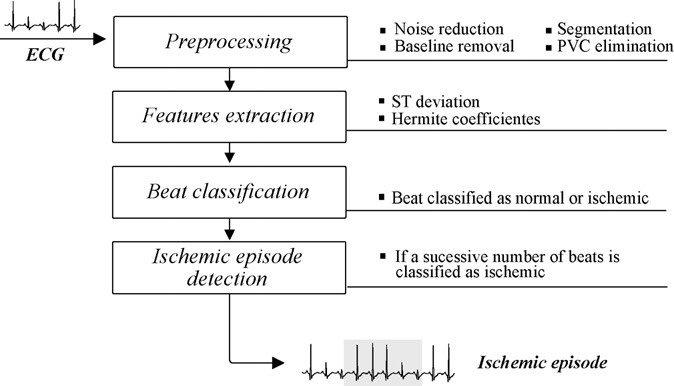
\includegraphics[width=0.9\textwidth]{figures/rocha_01.png}
    \caption{Diagrama de blocos da estratégia utilizada no método de Rocha et al. Extraído de \cite{Rocha10}}
    \label{fig:rocha_01}
\end{figure}

\subsection{Pré-processamento}
Nesta etapa, um sinal de entrada discreto contendo as amplitudes normalizadas\footnote{aqui, normalizado significa $(Amplitude - Deslocamento) / Ganho$} do ECG é processado para redução de ruído, segmentação em ondas características, eliminação de extra-sístoles ventriculares e, por último, remoção da linha de base.

A redução de ruído é alcançada com a aplicação de um filtro passa-baixas de Butterworth de 4\textordfeminine\ ordem e frequência de corte igual a 40Hz. O sinal filtrado é então submetido a um procedimento de segmentação, em que as ondas características de cada batida são identificadas. Seguindo a especificação de Rocha, utilizou-se para tal procedimento o algoritmo descrito em \cite{Sun05}, baseado em derivação morfológica multi-escala. Na saída obtêm-se as localizações de início, pico e fim de cada onda característica.

Após a segmentação, cada batida é classificada como normal ou extra-sístole ventricular (abreviada por PVC, do inglês \emph{premature ventricular contractions}). Para tal procedimento emprega-se o algoritmo proposto em \cite{Couceiro08}, que extrai 13 medidas das batidas e as usa como entrada numa rede neural. As PVCs são removidas da lista de batidas do ECG, e somente aquelas classificadas como normais serão analisadas nas etapas posteriores.

O último procedimento nesta etapa consiste em extrair do sinal de ECG a linha de base, e subtraí-la do próprio sinal afim de torná-lo mais próximo da linha isoelétrica. Isso é necessário para as próximas etapas, pois alguns procedimentos exigem que as batidas estejam bem alinhadas com o nível de amplitude zero.

\subsection{Extração de características}
Nesta etapa, dois grupos de características são extraídos do ECG, quais sejam, medida do desvio de segmento ST e expansão de Hermite do complexo QRS e das ondas T. Variações no desvio do segmento ST, medido a partir da linha de base, são usadas para discriminar as batidas isquêmicas das normais. De maneira similar, variações na morfologia do complexo QRS e da onda T indicam presença ou não de isquemia.

\subsubsection{Medida do desvio de segmento ST}
Para compor o primeiro grupo de características, duas medidas são obtidas através de dois métodos distintos. Um deles é baseado na localização dos picos de onda R, de acordo com o algoritmo proposto em \cite{Pang05}. O outro é derivado de uma análise tempo-frequencial do ECG usando a transformada de Wigner-Ville, conforme descrito abaixo.

A distribuição de Wigner-Ville de um sinal contínuo permite representar em detalhes a distribuição dos componentes espectrais do sinal no eixo temporal. Ela pode ser definida pela equação abaixo.
\begin{equation} \label{equ:wigner_ville}
    W_x(t,f) = \int_{-\infty}^{\infty} x\left( t+\frac{\tau}{2} \right) x^*\left( t-\frac{\tau}{2} \right) e^{-j2\pi f \tau} d\tau
\end{equation}
onde o termo dependente de $x$ é a função de autocorrelação instantânea, e o operador $^*$ indica o conjugado complexo. A correspondente em tempo discreto, chamada pseudo-transformada de Wigner-Ville, é dada pela equação abaixo.
\begin{equation} \label{equ:pseudo_wigner_ville}
    W_x(nT,f) = 2T\sum_{-L}^{L}x(n+p)x^*(n-p)w(p)w^*(-p)e^{-j4\pi f\tau}
\end{equation}

Nesta equação, $T$ é o período de amostragem e $w$ é uma janela simétrica de largura $2L+1$. Os autores não estabelecem um valor para $L$, mas dizem que deve ser maior que o número de amostras contidas em um complexo QRS, para garantir que as características do formato de onda não sejam perdidas na transformação. Portanto, adaptou-se o algoritmo para tomar uma janela de largura 32, que é maior do que o número de amostras em $100ms$ do sinal quando amostrado a uma taxa $F_S = 250 Hz$ (todos os registros de ECG usados para testar este algoritmo possuem taxa de amostragem igual a 250 Hz).

Após a transformação, soma-se os valores absolutos das componentes de baixa frequência do sinal em dois intervalos de tempo distintos: um à esquerda do pico de onda R, e outro à direita do mesmo ponto. O resultado provê informações sobre a concentração de energia nos dois intervalos, e o que se busca é o ponto mínimo em cada um deles. O ponto mínimo à esquerda é o chamado ponto isoelétrico, enquanto o ponto mínimo à direita é chamado ponto J. Estes conceitos são discutidos em detalhe em \cite{Rocha10}, mas é suficiente aqui mencionar que a medida do desvio ST é a diferença entre as amplitudes nos pontos J e isoelétricos: $Signal(J_k) - Signal(I_k)$, onde $k$ é o índice da batida.

\subsubsection{Caracterização do complexo QRS e da onda T}
Para o segundo grupo de características, os autores propuseram uma técnica baseada em funções de Hermite. Uma função de Hermite de ordem $n$ pode ser expressa como o produto de uma Gaussiana com um polinômio de Hermite, conforme a equação abaixo.
\begin{equation} \label{equ:hermite_function}
    H^n(t,l) = \frac{e^{-t^2/2l^2}}{\sqrt{n!2^n\sqrt{\pi}l}}p^n\left(\frac{t}{l}\right)
\end{equation}
onde $p^n$ é o polinômio de Hermite de ordem $n$ e $l$ é um fator de escala.

Usando esta definição, e sabendo que as funções de Hermite formam uma base para o espaço de funções integráveis ao quadrado ($L^2$), é possível aproximar um sinal discreto por uma expansão em funções de Hermite. A expansão consiste em obter uma lista de coeficientes que satisfazem a equação abaixo.
\begin{equation} \label{equ:hermite_expansion}
   \hat{y}(k) = \sum_{j=0}^{m-1} c_jH^j(k,l)
\end{equation}
onde $c_j$ é o coeficiente da $j$-ésima função de Hermite e $m$ é o número de funções utilizadas na aproximação ($m$ deve ser menor ou igual ao número de amostras do sinal de entrada, $N$). Os coeficientes são solução da equação abaixo.
\begin{equation} \label{equ:solve}
    C = (H^TH)^{-1}H^TY
\end{equation}
onde H é uma matriz formada pelas funções de Hermite,
\begin{equation}
    H = [H_0\ H_1\ \cdots\ H_{m-1}]
\end{equation}
C é um vetor coluna contendo os $m$ coeficientes de Hermite
\begin{equation}
    C = [c_0\ c_1\ \cdots\ c_{m-1}]^T
\end{equation}
e Y é um vetor coluna de tamanho $N$ contendo as amplitudes do sinal de entrada.

No algoritmo proposto, o sinal é separado em dois componentes: um contendo as amostras do complexo QRS e o outro, as da onda T. Essa separação permite aproximar melhor o formato de uma batida cardíaca, já que o complexo QRS e a onda T diferem morfologicamente, além de estarem bastante separados temporalmente. Entretanto, apenas as primeiras seis funções de Hermite são consideradas ($m = 6$), com o objetivo de minimizar custos computacionais. Assim, para cada batida, dois conjuntos de amostras ($Y_{QRS}$ e $Y_{ST-T}$) são submetidos ao procedimento de expansão de Hermite, e a saída nos fornece uma lista de 6 coeficientes para o primeiro conjunto ($C_{QRS}$) e uma lista de 6 coeficientes para o segundo ($C_{ST-T}$).

É importante salientar que o domínio das funções de Hermite varia de acordo com o número de amostras do sinal de entrada. Na implementação, um tamanho fixo foi definido, grande o suficiente para suportar todas as possíveis larguras das ondas presentes em um sinal de ECG. A matriz correspondente pode então ser construída antes do processamento e, dessa forma, apenas as linhas necessárias da matriz são acessadas e utilizadas no cálculo dos coeficientes.

\subsection{Código MATLAB}
No código-fonte \ref{lst:rocha} pode ser visualizado um trecho que compõe a rotina principal do método implementado. O sinal de entrada e sua taxa de amostragem provêm de uma base de dados, sendo que as amplitudes são normalizadas antes do início da rotina. Com exeção das funções \texttt{ecg\_find\_close\_beats} e \texttt{compute\_statistics}, todas fazem parte de um conjunto de rotinas criadas especialmente para o método de Rocha et al.

\lstinputlisting[
    label={lst:rocha},
    caption={Trecho extraído do arquivo rocha.m}
]{listings/rocha.m}
